\chapter{Priprava na 7. laboratorijske vaje}
\section{Ločenje preklopnih funkcij}

Ločenje preklopne funkcije po spremenljivki $x_i$ je definirano z izrazom

\begin{align*}
&f(x_1, x_2,..., x_{i-1}, x_i, x_{i+1},..., x_n) = \\ &f(x_1, x_2,..., x_{i-1}, 0, x_{i+1},..., x_n) \ol x_i \vee f(x_1, x_2,..., x_{i-1}, 1, x_{i+1},..., x_n) x_i 
\end{align*}

za ločenje konjunktivnih izrazov in z izrazom

\begin{align*}
&f(x_1, x_2,..., x_{i-1}, x_i, x_{i+1},..., x_n) = \\ &(f(x_1, x_2,..., x_{i-1}, 0, x_{i+1},..., x_n) \vee x_i) (f(x_1, x_2,..., x_{i-1}, 1, x_{i+1},..., x_n) \vee \ol x_i) 
\end{align*}

za ločenje disjunktivnih izrazov. Pri tem funkcijama, ki nastopata v izrazu, pravimo \emph{funkcijska ostanka}:

$$
f_0(x_1, x_2,..., x_{i-1}, x_{i+1},..., x_n) = f(x_1, x_2,..., x_{i-1}, 0, x_{i+1},..., x_n),
$$

$$
f_1(x_1, x_2,..., x_{i-1}, x_{i+1},..., x_n) = f(x_1, x_2,..., x_{i-1}, 1, x_{i+1},..., x_n).
$$

Za realizacijo preklopnih funkcij z multiplekserji uporabljamo konjunktivno ločevanje izrazov, zato bomo
v nadaljevanju obravnavali le tega.

\begin{zgled}
\label{zgled:ostanki}
Funkcijo $f(x_1, x_2, x_3) = \vee^3(0, 2, 5, 6, 7)$ loči preko spremenljivke $x_1$.
\end{zgled}
\begin{resitev}

Funkcijo lahko zapišemo kot:

\begin{align*}
	f(x_1, x_2, x_3)& = &\ol x_1 \ol x_2 \ol x_3 \vee \ol x_1 x_2 \ol x_3 \vee x_1 \ol x_2 x_3 \vee x_1 x_2 \ol x_3 \vee x_1 x_2 x_3\\
	 & = &(\ol 0 \ol x_2 \ol x_3 \vee \ol 0 x_2 \ol x_3 \vee 0 \ol x_2 x_3 \vee 0 x_2 \ol x_3 \vee 0 x_2 x_3) \ol x_1 \vee\\
	&    &\vee (\ol 1 \ol x_2 \ol x_3 \vee \ol 1 x_2 \ol x_3 \vee 1 \ol x_2 x_3 \vee 1 x_2 \ol x_3 \vee 1 x_2 x_3) x_1 \\
	& = &(\ol x_2 \ol x_3 \vee x_2 \ol x_3)\ol x_1 \vee (\ol x_2 x_3 \vee x_2 \ol x_3 \vee x_2 x_3) x_1
\end{align*}

\bigskip

Pri tem dobimo funkcijska ostanka:
\begin{align*}
&f_0(x_2,x_3)=\ol x_2 \ol x_3 \vee x_2 \ol x_3\\
&f_1(x_2,x_3)=\ol x_2 x_3 \vee x_2 \ol x_3 \vee x_2 x_3
\end{align*}

\bigskip

Ločimo funkcijski ostanek $f_0(x_2, x_3)$ še po $x_2$:
\begin{align*}
f_0(x_2,x_3)&=(\ol 0 \ol x_3 \vee 0 \ol x_3)\ol x_2 \vee (\ol 1 \ol x_3 \vee 1 \ol x_3) x_2\\
&=\ol x_3\ol x_2 \vee \ol x_3 x_2
\end{align*}

\bigskip

Pri tem dobimo funkcijska ostanka:
\begin{align*}
&f_{00}(x_3)=\ol x_3\\
&f_{01}(x_3)=\ol x_3
\end{align*}

\bigskip

Ločimo funkcijski ostanek $f_1(x_2, x_3)$ še po $x_2$:
\begin{align*}
f_1(x_2,x_3)&=(\ol 0 x_3 \vee 0 \ol x_3 \vee 0 x_3)\ol x_2 \vee (\ol 1 x_3 \vee 1 \ol x_3 \vee 1 x_3) x_2\\
&=x_3\ol x_2 \vee (\ol x_3 \vee x_3) x_2\\
&=x_3\ol x_2 \vee 1x_2
\end{align*}

\bigskip

Pri tem dobimo funkcijska ostanka:
\begin{align*}
&f_{10}(x_3)=x_3\\
&f_{11}(x_3)=1
\end{align*}

\end{resitev}

\section{Multiplekser}
Multiplekser spada v družino strukturalnih preklopnih vezij. Multiplekser ima dva niza vhodnih spremenljivk, in sicer \emph{naslovne spremenljivke} na naslovnih vhodih ($A_n,A_{n-1},...,A_0$) in \emph{podatkovne spremenljivke} na podatkovnih vhodih ($I_0, I_1,..., I_{2^n-1}$). Na podlagi vrednosti naslovnih spremenljivk se izbere podatkovni vhod, ki se bo preslikal na izhod multiplekserja. Multiplekser v kombinaciji s konstanto 0 ali 1 predstavlja funkcijsko poln sistem - z njim oziroma s kombinacijo več multiplekserjev lahko realiziramo poljubno logično funkcijo.\\

Multiplekser v odvisnosti od vrednosti naslovnih vhodov na izhod preslika enega izmed podatkovnih vhodov. Natančneje, na izhod se preslika podatkovni vhod z indeksom, ki je enak desetiškemu zapisu vrednosti na naslovnih vhodih. Splošno delovanje multiplekserja prikazuje tabela \ref{tab:mux_2n1}.\\

\begin{table}[h]
\begin{center}
\begin{tabular}{cccc|c}
$A_{n-1}$ & $A_{n-2}$ & $...$ & $A_{0}$ &  $f$ \\
\hline
0 & 0 & ... & 0 & $I_0$  		\\
0 & 0 & ... & 1 & $I_1$  		\\
. & . & ... & . & .						\\
. & . & ... & . & .						\\
. & . & ... & . & .						\\
1 & 1 & ... & 0 & $I_{2^n-2}$ \\
1 & 1 & ... & 1 & $I_{2^n-1}$ \\
\end{tabular}
\caption{Splošno delovanje multiplekserja MUX $2^n/1$.}
\label{tab:mux_2n1}
\end{center}
\end{table}

Multiplekser z $n$ naslovnimi spremenljivkami označujemo kot MUX $2^n/1$. Realizacijo funkcije z multiplekserjem praviloma podajamo z logično shemo. Splošno logično shemo za multiplekser MUX $2^n/1$
prikazuje slika \ref{fig:mux_2n1}.

\begin{figure}[ht]
\centering
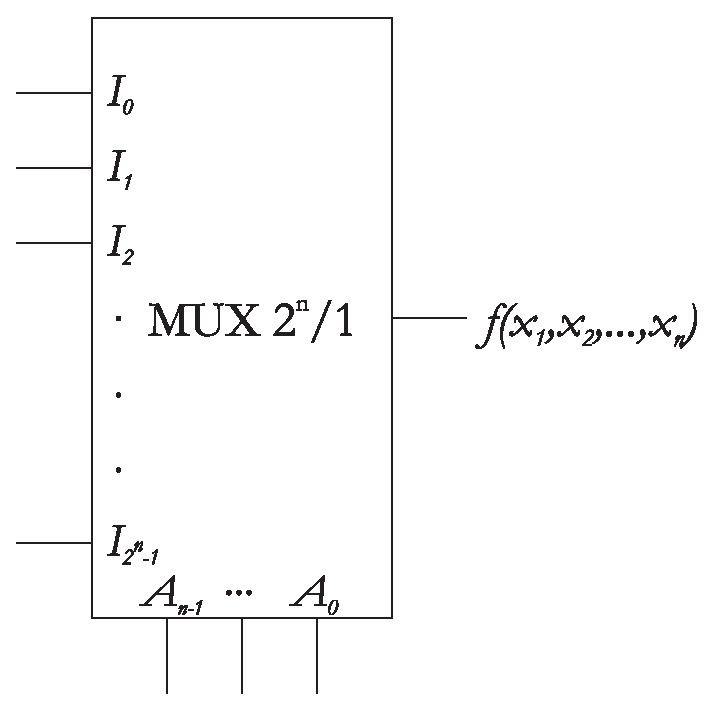
\includegraphics[width=0.5\linewidth]{mux-1.eps}
\caption{Splošna logična shema za multiplekser MUX $2^n/1$.}
\label{fig:mux_2n1}
\end{figure}

\section{Realizacija preklopnih funkcij z multiplekserji}

Z uporabo konstant 0 in 1 in multiplekserja MUX $2^n/1$ lahko realiziramo poljubno preklopno funkcijo z $n+1$ vhodnimi spremenljivkami. Realizacija funkcij z uporabo multiplekserjev z manjšim številom naslovnih vhodov poteka z drevesno oziroma kaskadno vezavo multiplekserjev.\\

Realizacija preklopnih funkcij z multiplekserji poteka na podlagi ločenja. Funkcijo ločimo preko vhodnih spremenljivk, ki jih vežemo na naslovne vhode, na podatkovnih vhodih pa realiziramo funkcijske ostanke.\\

V nadaljevanju bomo demonstrirali realizacijo funkcije $f(x_1, x_2, x_3) = \vee^3(0, 2, 5, 6, 7)$ z multiplekserji različnih velikosti.

\subsection{Število vhodnih spremenljivk je enako številu naslovnih vhodov multiplekserja}

Na razpolago imamo konstanti 0 in 1 in multiplekser, ki ima enako število naslovnih vhodov, kot je število vhodnih spremenljivk preklopne funkcije. V tem primeru na podatkovne vhode vežemo funkcijske vrednosti v enakem vrstnem redu kot ti nastopajo v pravilnostni tabeli, na naslovne vhode pa vhodne spremenljivke - prav tako v enakem vrstnem redu kot nastopajo v pravilnostni tabeli. Funkcijo torej ločimo preko vseh vhodnih spremenljivk, zato lahko vse funkcijske ostanke izrazimo s konstantami 0 in 1.

\begin{zgled}
Realiziraj funkcijo $\vee^3(0,2,5,6,7)$ z MUX $8/1$.
\end{zgled}
\begin{resitev}
V prvem koraku zapišemo pravilnostno tabelo funkcije.

\begin{center}
\begin{tabular}{ccc|c}
$x_1$ & $x_2$ & $x_3$ &  $f(x_1,x_2,x_3)$ \\
\hline
0 & 0 & 0 & 1 \\
0 & 0 & 1 & 0 \\
0 & 1 & 0 & 1 \\
0 & 1 & 1 & 0 \\
1 & 0 & 0 & 0 \\
1 & 0 & 1 & 1 \\
1 & 1 & 0 & 1 \\
1 & 1 & 1 & 1 \\
\end{tabular}
\end{center}

\bigskip

V drugem koraku na podatkovne vhode vežemo funkcijske vrednosti v enakem vrstnem redu kot ti nastopajo v pravilnostni tabeli, na naslovne vhode pa vhodne spremenljivke - prav tako v enakem vrstnem redu kot nastopajo v pravilnostni tabeli (glej sliko \ref{fig:mux_zgled_1}).

\bigskip
\begin{figure}[ht]
\centering
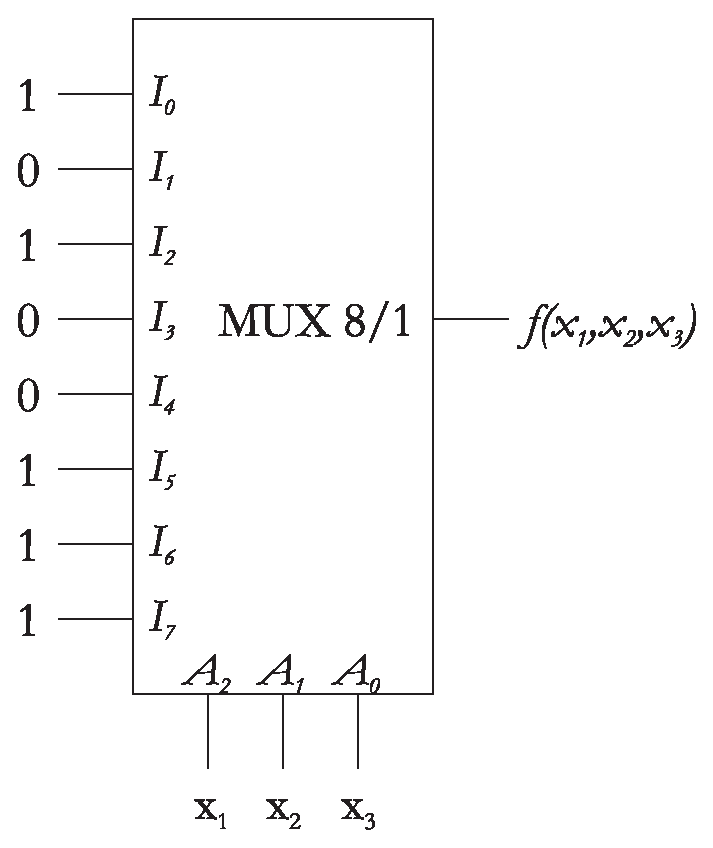
\includegraphics[width=0.5\linewidth]{mux-2.eps}
\caption{Realizacija 3-vhodne funkcije z multiplekserjem MUX $8/1$.}
\label{fig:mux_zgled_1}
\end{figure}

\end{resitev}

\subsection{Število vhodnih spremenljivk je za 1 večje od števila naslovnih vhodov multiplekserja}

Na razpolago imamo konstanti 0 in 1 in  multiplekser, ki ima število naslovnih vhodov za 1 manjše, kot je število vhodnih spremenljivk preklopne funkcije. Funkcijo ločimo po spremenljivkah glede na njihov vrstni red od leve proti desni. Iz tega sledi, da skrajno leve vhodne spremenljivke vežemo na naslovne vhode multiplekserja (najbolj levo spremenljivko na naslovni vhod z najvišjim indeksom). Na podatkovnih vhodih realiziramo funkcijski ostanek, ki ga lahko vedno izrazimo z najmanj pomembno vhodno spremenljivko, njeno negacijo, konstanto 0 in konstanto 1.

\begin{zgled}
Realiziraj funkcijo $\vee^3(0,2,5,6,7)$ z MUX $4/1$.\\
\end{zgled}
\begin{resitev}

V prvem koraku zapišemo pravilnostno tabelo funkcije.

\bigskip
\begin{center}
\begin{tabular}{ccc|cc}
$x_1$ & $x_2$ & $x_3$ &  $f(x_1,x_2,x_3)$ \\
\hline
0 & 0 & 0 & 1 &\multirow{2}{*}{$I_0=\ol x_3$}\\
0 & 0 & 1 & 0 &\\ 
\hline
0 & 1 & 0 & 1 &\multirow{2}{*}{$I_1=\ol x_3$}\\
0 & 1 & 1 & 0 &\\
\hline
1 & 0 & 0 & 0 &\multirow{2}{*}{$I_2=x_3$}\\
1 & 0 & 1 & 1 &\\
\hline
1 & 1 & 0 & 1 &\multirow{2}{*}{$I_3=1$}\\
1 & 1 & 1 & 1 &\\
\end{tabular}
\end{center}

\bigskip

V drugem koraku na naslovne vhode vežemo najpomembnejše spremenljivke (v našem primeru $x_1$ in $x_2$). V našem primeru na vhod $A_1$ vežemo $x_1$, na vhod $A_2$ pa $x_2$. S tem funkcijo ločimo preko spremenljivk $x_1$ in $x_2$. S pomočjo spremenljivke, ki je ostala, uporabe negacij, konstante 0 in 1, realiziramo funkcijske ostanke ločenja, ki jih vežemo na podatkovne vhode (glej sliko \ref{fig:mux_zgled_2}).

\end{resitev}


\bigskip
\begin{figure}[ht]
\centering
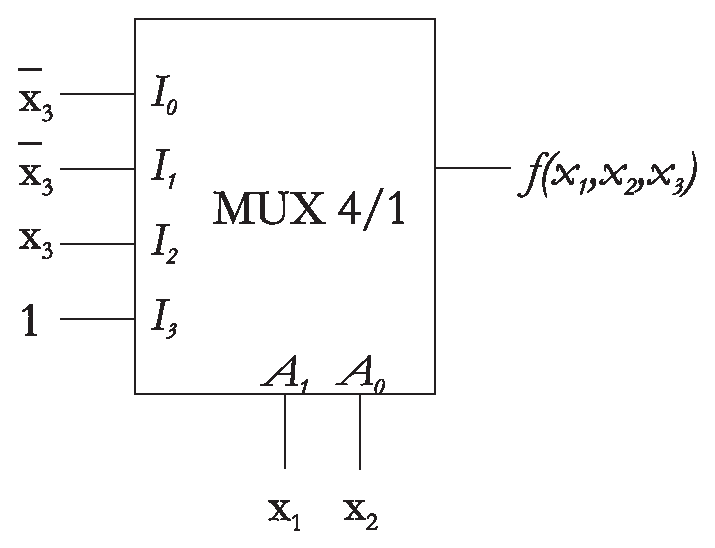
\includegraphics[width=0.5\linewidth]{mux-3.eps}
\caption{Realizacija 3-vhodne funkcije z multiplekserjem MUX $4/1$.}
\label{fig:mux_zgled_2}
\end{figure}

\subsection{Število vhodnih spremenljivk je za več kot 1 večje od števila naslovnih vhodov multiplekserja}

Če je število vhodnih spremenljivk funkcije za več kot za 1 večje od števila naslovnih vhodov multiplekserja, moramo za realizacijo uporabiti večje število multiplekserjev, ki jih med seboj vežemo v drevesno (kaskadno) vezavo. Ponavadi funkcijo ločimo po najpomembnejših spremenljivkah, ni pa to pravilo. V tem primeru začnemo z vezavo najpomembnejših spremenljivk na naslovne vhode zadnjega multiplekserja v kaskadi.

\begin{zgled}

Realiziraj funkcijo $\vee^3(0,2,5,6,7)$ z MUX $2/1$.\\

\end{zgled}
\begin{resitev}

V prvem koraku zapišemo pravilnostno tabelo in funkcijo
\begin{itemize}
\item najprej ločimo po $x_1$,
\item zgornji del (funkcijski ostanek pri $x_1=0$) lahko izrazimo z $\ol x_3$,
\item spodnji del (funkcijski ostanek pri $x_1=1$) ločimo še po $x_2$ (zgornji del, t.j. funkcijski ostanek pri $x_2 = 0$, lahko izrazimo z $x_3$, spodnji del, t.j. funkcijski ostanek pri $x_2 = 1$, pa s konstanto 1).
\end{itemize}

\bigskip

Ostanke pri ločenju smo izračunali že v zgledu \ref{zgled:ostanki}.

\begin{center}
\begin{tabular}{ccc|cc}
$x_1$ & $x_2$ & $x_3$ &  $f(x_1,x_2,x_3)$ \\
\hline
0 & 0 & 0 & 1 & \multirow{4}{*}{$\ol x_3$}\\
0 & 0 & 1 & 0 &\\ 
0 & 1 & 0 & 1 &\\
0 & 1 & 1 & 0 &\\
\hline
1 & 0 & 0 & 0 & \multirow{2}{*}{$x_3$}\\
1 & 0 & 1 & 1 &\\
\hline
1 & 1 & 0 & 1 & \multirow{2}{*}{$1$}\\
1 & 1 & 1 & 1 &\\
\end{tabular}
\end{center}

\bigskip

V drugem koraku narišemo shemo realizacije. Ker smo tabelo najprej ločili po $x_1$, $x_1$ uporabimo kot naslovni vhod zadnjega multiplekserja v kaskadi. Funkcijski ostanek $f_0$ po $x_1$ lahko izrazimo z $x_3$ -- $\ol x_3$ vežemo na podatkovni vhod $I_0$ multiplekserja. Spodnjega dela, ki predstavlja funkcijski ostanek $f_1$ po $x_1$, ne moremo izraziti na enostaven način, zato ga ločimo še po spremenljivki $x_2$ in za njegovo realizacijo uporabimo dodaten multiplekser MUX $2/1$. Le-tega vežemo na vhod $I_1$ zadnjega multiplekserja v kaskadi. Na naslovni vhod dodatnega multiplekserja vežemo spremenljivko $x_2$. Funkcijski ostanek $f_0$ ločenja po $x_2$ lahko izrazimo z $x_3$, ostanek $f_1$ pa s konstanto $1$ - razvidno iz tabele. Na podatkovni vhod $I_0$ dodatnega multiplekserja torej vežemo $x_3$, na vhod $I_1$ pa konstanto $1$. Realizacijo prikazuje slika \ref{fig:mux_zgled_3}.

\begin{figure}[ht]
\centering
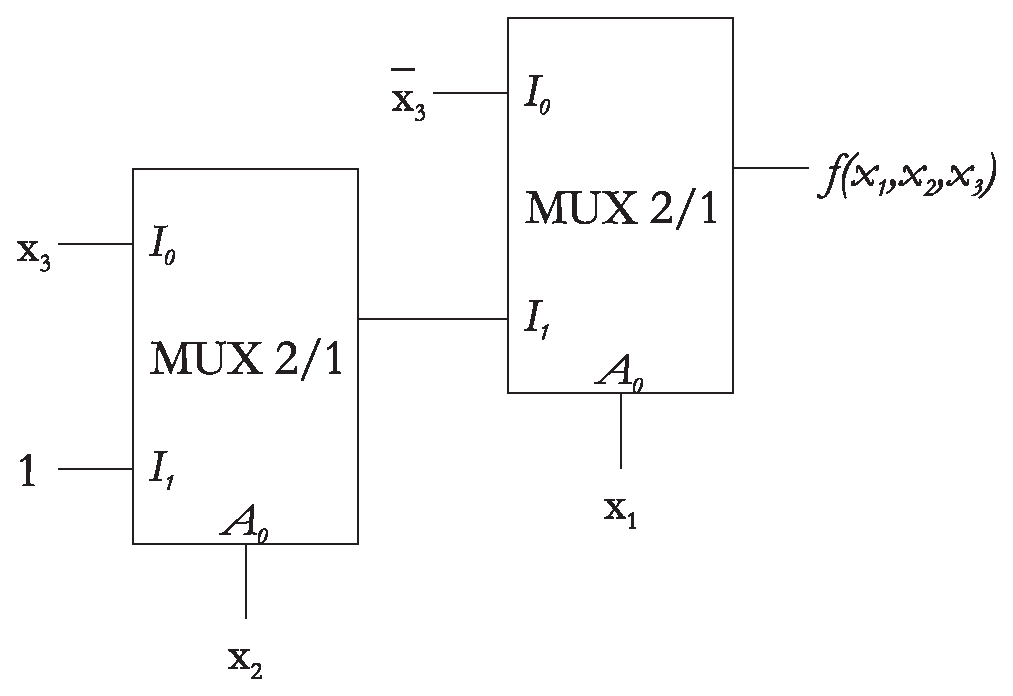
\includegraphics[width=0.75\linewidth]{mux-4.eps}
\caption{Realizacija 3-vhodne preklopne funkcije z dvema multiplekserjema MUX $2/1$.}
\label{fig:mux_zgled_3}
\end{figure}

\end{resitev}

%\section*{Laboratorijske vaje}
%Z uporabo multiplekserjev MUX 4/1 in MUX 2/1 v Logisimu realiziraj preklopno funkcijo $f(x_1,x_2,x_3,x_4) = x_1 \overline x_2 \rightarrow x_3 x_4$.
%
%\bigskip
%\begin{tabular}{cccc|c|c}
%$x_1$ & $x_2$ & $x_3$ & $x_4$ & $f$ & I\\
%\hline
%0 & 0 & 0 & 0 & 1 & \multirow{2}{*}{1}\\
%0 & 0 & 0 & 1 & 1 &\\
%\hline
%0 & 0 & 1 & 0 & 1 & \multirow{2}{*}{1}\\
%0 & 0 & 1 & 1 & 1 &\\
%\hline
%0 & 1 & 0 & 0 & 1 & \multirow{2}{*}{1}\\
%0 & 1 & 0 & 1 & 1 &\\
%\hline
%0 & 1 & 1 & 0 & 1 & \multirow{2}{*}{1}\\
%0 & 1 & 1 & 1 & 1 &\\
%\hline\hline
%1 & 0 & 0 & 0 & 0 & \multirow{2}{*}{0}\\
%1 & 0 & 0 & 1 & 0 &\\
%\hline
%1 & 0 & 1 & 0 & 0 & \multirow{2}{*}{$x_4$}\\
%1 & 0 & 1 & 1 & 1 &\\
%\hline
%1 & 1 & 0 & 0 & 1 & \multirow{2}{*}{1}\\
%1 & 1 & 0 & 1 & 1 &\\
%\hline
%1 & 1 & 1 & 0 & 1 & \multirow{2}{*}{1}\\
%1 & 1 & 1 & 1 & 1 &\\
%\end{tabular}
%
%
%
%\bigskip
%\begin{figure}[ht]
%\centering
%\includegraphics[width=0.75\linewidth]{slika_v7_1.eps}
%\end{figure}